% Copyright 2021 Edoardo Riggio

% Licensed under the Apache License, Version 2.0 (the "License");
% you may not use this file except in compliance with the License.
% You may obtain a copy of the License at

% 	http://www.apache.org/licenses/LICENSE-2.0

% Unless required by applicable law or agreed to in writing, software
% distributed under the License is distributed on an "AS IS" BASIS,
% WITHOUT WARRANTIES OR CONDITIONS OF ANY KIND, either express or implied.
% See the License for the specific language governing permissions and
% limitations under the License.

\documentclass{article}

\usepackage{hyperref, amsmath, graphicx, amssymb, csquotes, listings}
\usepackage{fancyvrb,newverbs,xcolor}

\graphicspath{ {./assets/} }

\definecolor{cverbbg}{gray}{0.93}

\newenvironment{cverbatim}
 {\SaveVerbatim{cverb}}
 {\endSaveVerbatim
  \flushleft\fboxrule=0pt\fboxsep=.5em
  \colorbox{cverbbg}{\BUseVerbatim{cverb}}%
  \endflushleft
}

\newenvironment{lcverbatim}
 {\SaveVerbatim{cverb}}
 {\endSaveVerbatim
  \flushleft\fboxrule=0pt\fboxsep=.5em
  \colorbox{cverbbg}{%
    \makebox[\dimexpr\linewidth-2\fboxsep][l]{\BUseVerbatim{cverb}}%
  }
  \endflushleft
}

\newcommand{\ctexttt}[1]{\colorbox{cverbbg}{\texttt{#1}}}
\newverbcommand{\cverb}
  {\setbox\verbbox\hbox\bgroup}
  {\egroup\colorbox{cverbbg}{\box\verbbox}}
  
\lstdefinestyle{c++}{
  frame=single, language={C++}, numbers=left, numberstyle=\tiny, tabsize=4, breaklines=true,
  basicstyle=\ttfamily\scriptsize,
  keywordstyle=\color{blue}\ttfamily,
  otherkeywords={WIDTH},
  keywords=[2]{__shared__},
  keywordstyle=[2]\color{orange}\ttfamily,
  stringstyle=\color{red}\ttfamily,
  commentstyle=\color{green}\ttfamily
}

\begin{document}
\begin{titlepage}
    \begin{center}
        \vspace*{1cm}
        
        \Huge
        \textbf{Computer Graphics Cheatsheet}
        
        \vspace{0.5cm}
        \LARGE
        
        \vspace{.5cm}
        
        Edoardo Riggio
   		  \vspace{1.5cm}
       
        \vfill
        
        \today
        
        \vspace{.8cm}
          \Large
          Computer Graphics - S.A. 2021 \\
        Computer Science\\
        Universit\`{a} della Svizzera Italiana, Lugano\\
        
    \end{center}
\end{titlepage}

\tableofcontents

\newpage

\section{Ray Tracing}
\textbf{Ray tracing} is a method of graphics rendering that simulates the physical behaviour of light.

\subsection{Whitted Ray Tracing}
One ray is traced for every single pixel. These are known as the \textbf{primary rays}. \\ \\
For each of the rays, we need to find their intersection with the scene. After we do so, secondary rays can be generated. Such rays are:

\begin{itemize}
	\item Shadow Ray
	\item Reflection Ray
	\item Refraction Ray
\end{itemize}
The color of each of the pixels is determined based on the aggregated color of the rays.

\begin{center}
	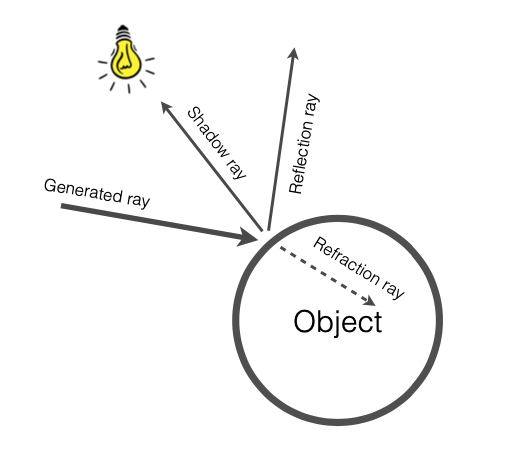
\includegraphics[width=5cm]{whitted_rt.png}
\end{center}
The secondary rays are recursively generated. Some termination conditions for this generation are:

\begin{itemize}
	\item Ray leaves the scene without ever hitting an object
	\item Maximal recursion depth is reached
	\item Contribution of the ray to the final color is negligible
\end{itemize}

\subsection{Camera / Image Definition}
We are considering a global coordinate system for the raytracer. Some of the characteristics of the \textbf{camera} are:

\begin{itemize}
	\item It is located at the origin $(0, 0, 0)$
	\item It has a horizontal opening $\alpha$, the FOV (Field Of View)
\end{itemize}
Some of the characteristics of the \textbf{image} are:

\begin{itemize}
	\item Image plane is located at $z = 1$
	\item Resolution of the image is of $w \cdot h$ pixels
	\item Pixels have indices $(i, j)$ and coordinates $p_{ij} = (x_{ij}, y_{ij}, z_{ij})$
\end{itemize}

\begin{center}
	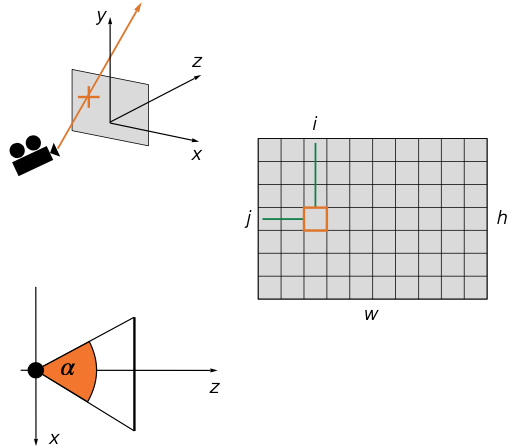
\includegraphics[width=6cm]{scene_def.png}
\end{center}

\subsection{Ray Computation}
The equation of a \textbf{ray} is the following:

\[ \gamma(t) = o + dt \] \\
Where $t$ is the distance between the origin and the intersection with an object, $o$ is the point representing the camera position, and $d$ is the vector representing the viewing direction -- of magnitude 1.

\begin{center}
	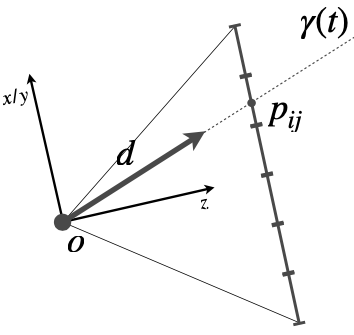
\includegraphics[width=5cm]{ray_comp.png}
\end{center} 
In order to compute the vector $d$, we need to do the following:

\begin{lstlisting}[style=c++]
s = (2 * tan(alpha / 2)) / 2;
X = (-w * s) / 2;
Y = (h * s) / 2;

for (int i = 0; i++; i < w) {
	for (int j = 0; j++; j < h) {
		dx = X + (i * s) + (0.5 * s);
		dy = Y - (j * s) - (0.5 * s);
		dz = 1;
		
		d = glm::vec3(dx, dy, dz);
		d = glm::vec3.normalize(d)
	}
}
\end{lstlisting}

\subsection{Ray-Sphere Intersection}
In order to define a \textbf{sphere}, we need to set the centre and the radius. Once that is done, we need to check is the sphere intersects with the generated ray. To do so we need to check if there is some $t$ such that:

\[ ||~\gamma(t) - c~|| = r \] \\
In order to find the $t$, we use the following procedure.
\begin{align*}
	a & = \langle c, d \rangle \\
	D & = \sqrt{||~c~||^2 - \langle c, d \rangle^2} \\
	t_{1,2} & = \langle c,d \rangle \pm \sqrt{r^2 - D^2}
\end{align*}
If the ray intersects the sphere and the camera is not inside of the sphere, then the pixel corresponding to the intersection is painted.

\section{Lighting Models}
In order to compute the color values on an object's surface we can use rules based on the laws of physics -- radiometry and photometry. These rules model the effect of:

\begin{itemize}
	\item \textbf{Light Sources}
	\vspace{.2cm} \\
	Position, intensity and colour.
	
	\item \textbf{Object Surface}
	\vspace{.2cm} \\
	Geometry and reflective properties.
\end{itemize}

\subsection{Illumination Factors}
The intensity of a color depends on several different factors:

\begin{itemize}
	\item The colour and reflective properties of the object
	\item The position and intensity of the light sources
	\item The position of the viewer
	\item The normal of the surface at point $p$
	\item The distance of point $p$ to the light source
\end{itemize}

\subsection{Components of the Phong Lighting Model}
These components are the \textbf{diffuse reflection}, the \textbf{ambient illumination}, and the \textbf{specular highlight}.

\subsubsection{Diffuse Reflection}
This type of reflection simulates Lambertian surfaces -- i.e. matte surfaces. Here the reflected light is dispersed evenly in all directions. \\ \\
There is also a material-dependent reflection constant $\rho_d \leq 1$. This is called the \textbf{diffuse coefficient}.

\begin{center}
	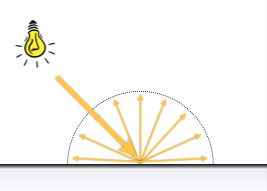
\includegraphics[width=4cm]{lambertian_surf.png}
\end{center}
The intensity $I_d$ of a surface coming from the diffuse reflection is proportional to the cosine of the angle between the surface normal $n$ and the direction of the light source $l$. This is known as the \textbf{Lambertian Cosine Rule}.

\begin{center}
	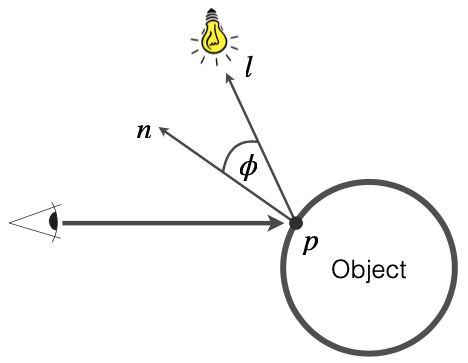
\includegraphics[width=5cm]{cos_rule.png}
\end{center}
The proper computation of the diffuse reflection is the following -- in which the Cosine Rule is applied:
\begin{align*}
	I_d &= \rho_d \cdot \cos\phi \cdot I \\
	&= \rho_d \cdot \langle n, l \rangle \cdot I
\end{align*}
Where $\rho_d$ is the diffuse coefficient, $n$ is the normal of the surface at point $p$, $l$ is the vector pointing towards the light source, and $I$ is the intensity of the light. \\ \\
An important thing to always check is that $\langle n, l \rangle > 0$.

\subsubsection{Ambient Illumination}
Ambient illumination is used in order to simulate indirect lighting. This refers to the effect of multiple inter-reflections of light between all objects, and to the isotropy and independence of light sources and viewpoints. \\ \\
There is a global constant $I$, and a material-dependent reflection constant $\rho_a \leq 1$. This is called the \textbf{ambient coefficient}. \\ \\
The ambient illumination is given by the following formula:

\[ I_a = \rho_a \cdot I \] \\
Where $\rho_a$ is the ambient coefficient, and $I$ is the intensity of the ambient lighting.

\subsubsection{Specular Reflection}
Specular reflection is used in order to simulate shiny surfaces. The incoming light is reflected in exactly one reflect direction. \\ \\
The specular reflection makes use of something known as the reflection vector.

\begin{center}
	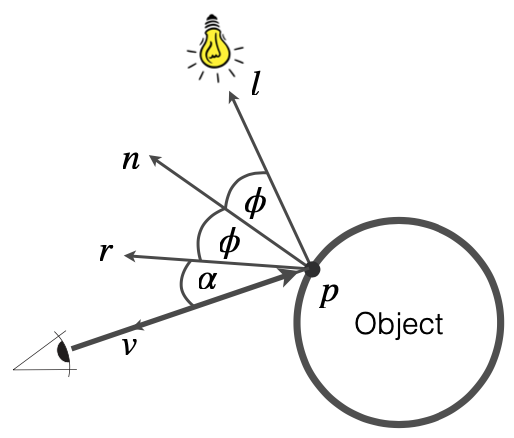
\includegraphics[width=5cm]{specular_refl.png}
\end{center}
The proper formulation of the specular reflection is the following:

\[ I_s = \rho_s \cdot \langle r, v \rangle^k \cdot I \] \\
Where $\rho_s$ is the specular coefficient of the object, $r$ is the reflection ray given by:

\[ r = 2n \cdot \langle n, l \rangle - l \] \\
Furthermore, $v$ is the viewing direction of the camera, $k \geq 1$ is the shininess coefficient, and $I$ is the light intensity.

\subsection{Phong Lighting Model}
The Phong lighting model is given by the superposition of ambient, diffuse, and specular terms for each light source. The final formula is the following:

\[ I = I_e + \rho_a \cdot I_a + \sum^n_{j = 1} (\rho_d \cdot \langle n, l_j \rangle + \rho_s \cdot \langle r_j, v \rangle^k) \cdot I_j \] \\
Where $I_e$ is the self-emitting intensity, $\rho_a$ is the diffuse coefficient, $I_a$ is the ambient intensity, $\rho_d$ is the diffuse coefficient, $n$ is the normal vector, $l$ is the vector pointing to the light source, $\rho_s$ is the specular coefficient, $r$ is the reflection ray, $v$ is the direction vector, $k$ is the shininess, and $I_j$ is the intensity of the $j$-th light source.

\subsection{Blinn-Phong Specular Reflection}
Here we use $h$ instead of $r$ in order to compute the specular reflection of an object.

\begin{center}
	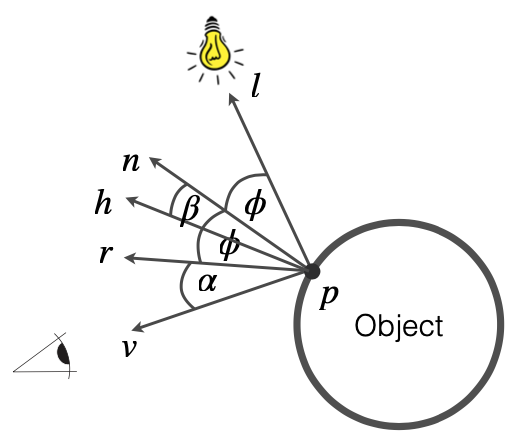
\includegraphics[width=5cm]{blinn_phong.png}
\end{center}
The proper formulation of the Blinn-Phong specular reflection is the following:

\[ I_s = \rho_s \cdot \langle n, h \rangle^{4k} \cdot I \] \\
Where $\rho_s$ is the specular coefficient, $n$ is the normal, $k$ is the shininess coefficient, $I$ is the light intensity, and $h$ is defined as:

\[ \frac{1}{2}(l + v) \] \\
Where $l$ is the light vector, and $v$ is the viewing direction.

\subsection{Light Sources}
\subsubsection{Point Light Sources}
\textbf{Point light sources} are a type of source that is isotropic -- radiates evenly in all directions, it is specified by a position, and has intensity $I$. \\ \\
\textbf{Directional light sources} are a special case of light sources which are only specified by direction. This is because it is an infinite set of rays that all have the same direction.

\subsubsection{Spot Light Sources}
This type of light source generates a light cone in a specified direction. In order to define the spot light source, we need to specify its position $p$, its direction $d$, and its opening angle $\Theta_L$.\\ \\
The intensity of the light is either maximal in the direction of $d$, or decreases following the formula:

\[ I'(\Theta) = \cos^k\Theta \cdot I \] \\
And it's 0 when $\Theta > \Theta_L$.

\subsection{Distance Attenuation}
The more the object is distant from the light source, the less it will be illuminated by the source. Its formal definition is:

\[ att(r) = \frac{1}{a_1 + a_2r + a_3r^2} \] \\
Where $r$ is the ray of light, and $a_1$, $a_2$, and $a_3$ are constant values.

\section{Light and Colour}
Light is composed of electrically charged particles undergoing acceleration, and emitting electromagnetic radiation. \\ \\
The eye has two different receptors in order to process such light:

\begin{itemize}
	\item \textbf{Rods}
	\vspace{.2cm} \\
	They perceive the intensity of light.
	
	\item \textbf{Cones}
	\vspace{.2cm} \\
	They perceive the colors. Three types of cones exist, one for the short wavelengths, one for the medium wavelengths, and one for the long wavelengths.
\end{itemize}

\subsection{Gamma Correction}
The relation between the display input and the intensity shown on the screen in non-linear. In order to account for this fact, we need to apply inverse gamma correction:

\[ I_{in} = I ^{\frac{1}{\gamma}} \] \\
Where $I_{in}$ is the input for our display, $I$ is the intensity computed by our raytracer, and $\gamma$ is a constant between $1.8$ and $2.4$. \\ \\
By doing so, we are basically assigning more bits to darker regions to which we are more sensitive.

\subsection{Tone Mapping}
It is impossible to reproduce the real luminance range onto a screen. For this reason we need to implement tone mapping.

\[ I_{in} = \max((\alpha \cdot I^\beta)^{\frac{1}{\gamma}}, 1.0) \] \\
Where $I_{in}$ is the input for our display, $I$ is the intensity computed by our raytracer, $\alpha$ and $\beta$ are the tone mapping coefficients, and $\gamma$ is the gamma coefficient.

\section{Triangle Meshes}
Complex surfaces can be approximated with triangle meshes. A triangle mesh is composed by the following elements:

\begin{itemize}
	\item \textbf{Vertices}
	\vspace{.2cm} \\
	Each vertex has three coordinates -- $x$, $y$, and $z$.
	
	\item \textbf{Edges}
	\item \textbf{Triangles/Faces}
	\vspace{.2cm} \\
	These are triplets of vertices which are displayed in counter-clockwise order.
\end{itemize}

\subsection{Ray-Triangle Intersection}
In order to compute the intersection between the ray and a triangle, we first need to compute the intersection between the ray and the triangle's plane. After, we do the following:

\begin{enumerate}
	\item Find a $t$ such that $p = \gamma(t)$ is coplanar with $p_1$, $p_2$ and $p_3$
	\item Check if $t > 0$ and that $p$ is inside of the triangle
	\item If the above conditions are all true, compute the lighting at point $p$. The normal vector at point $p$ is computed as:
	\[ n = (p_2 - p_1) \times (p_3 - p_1) \]
\end{enumerate}
In order to test whether the point is inside of the triangle, we use the \textbf{Barycentric Coordinates}.

\begin{center}
	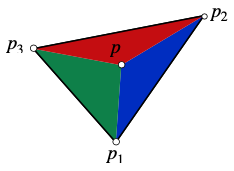
\includegraphics[width=4cm]{barycentric_coords.png}
\end{center}
The algorithm is the following:

\begin{enumerate}
	\item Consider a planar triangle made up of points $(p_1, p_2, p_3)$ and a point $p$
	\item Compute the area $W$ of the triangle
	\begin{align*}
		p_i &= (x_i, y_i, z_i) \\
		n &= (p_2 - p_1) \times (p_3 - p_1) \\
		2W &= ||n||
	\end{align*}		
	\item Compute the areas $w_1$, $w_2$ and $w_3$ of the triangles
	\begin{align*}
		p &= (x, y, z) \\
		n_i &= (p_{i+1} - p) \times (p_{i-1} - p) \\
		2w_i &= ||n_i|| \cdot \text{sign}(\langle n_i, n \rangle)
	\end{align*}
	\item Divide all of these areas by $W$. These values are $\lambda_1(p)$, $\lambda_2(p)$ and $\lambda_3(p)$ -- i.e. barycentric coordinates
	\[ \lambda_1(p) = \frac{w_1}{W} ~~~~~~~ \lambda_2(p) = \frac{w_2}{W} ~~~~~~~ \lambda_3(p) = \frac{w_3}{W} \]
\end{enumerate}
There are two properties for barycentric coordinates:

\begin{itemize}
	\item \textbf{Partition of Unity}
	\vspace{.2cm} \\
	The sum of all barycentric coordinates is equal to 1.
	
	\item \textbf{Non-Negativity}
	\vspace{.2cm} \\
	All of the barycentric coordinates are greater of equal to 0.
\end{itemize}

\section{Transformations}
There are two different ways of moving an object in the scene:

\begin{itemize}
	\item Moving the camera coordinates -- i.e. global coordinates
	\item Moving the object coordinates -- i.e. local coordinates
\end{itemize}
Each object is initially positioned at the origin of the scene. Here the local coordinates are the same as the global coordinates. Afterwards, the object is moved around using local coordinate system transformations.

\subsection{Homogeneous Coordinates}
In order to combine different transformations together, we need to work in four dimensions. Any point will be now written as:

\[ p = \begin{bmatrix} x \\ y \\ z \\ 1 \end{bmatrix} \] \\
Ad each displacement -- i.e. vector -- will be now written as:

\[ \overrightarrow{v} = \begin{bmatrix} x \\ y \\ z \\ 0 \end{bmatrix} \] \\
Such that:

\begin{itemize}
	\item $p + d = 1 + 0 = 1 =$ position
	\item $p - p = 1 - 1 = 0 =$ displacement
	\item $d + d = 0 + 0 = 0 =$ displacement
	\item $p + p = 1 + 1 = 0 =$ displacement
\end{itemize}

\subsection{Standard Transformations}
Some of the standard transformations we discussed are:

\begin{itemize}
	\item \textbf{Translation} by $t = (t_x, t_y, t_z)$
	\[ T = \begin{bmatrix} 1 & 0 & 0 & t_x \\ 0 & 1 & 0 & t_y \\ 0 & 0 & 1 & t_z \\ 0 & 0 & 0 & 1 \end{bmatrix} \]
	
	\item \textbf{Shearing} $yz$-plane, $xz$-plane and $xy$-plane
	\[ S_{yz} = \begin{bmatrix} 1 & 0 & 0 & 0 \\ d_y & 1 & 0 & 0 \\ d_z & 0 & 1 & 0 \\ 0 & 0 & 0 & 1 \end{bmatrix} ~~~~~ S_{xz} = \begin{bmatrix} 1 & d_x & 0 & 0 \\ 0 & 1 & 0 & 0 \\ 0 & d_z & 1 & 0 \\ 0 & 0 & 0 & 1 \end{bmatrix} ~~~~~ S_{xy} = \begin{bmatrix} 1 & 0 & d_x & 0 \\ 0 & 1 & d_y & 0 \\ 0 & 0 & 1 & 0 \\ 0 & 0 & 0 & 1 \end{bmatrix} \]
	
	\item \textbf{Scaling} by factors $s_x$, $s_y$, $s_z$
	\[ S = \begin{bmatrix} s_x & 0 & 0 & 0 \\ 0 & s_y & 0 & 0 \\ 0 & 0 & s_z & 0 \\ 0 & 0 & 0 & 1 \end{bmatrix} \]
	
	\item \textbf{Rotating} about axes $x$, $y$, $z$
	\[ R_x = \begin{bmatrix} 1 & 0 & 0 & 0 \\ 0 & \cos \alpha & -\sin \alpha & 0 \\ 0 & \sin \alpha & \cos \alpha & 0 \\ 0 & 0 & 0 & 1 \end{bmatrix} ~~~~~ R_y = \begin{bmatrix} \cos \alpha & 0 & \sin \alpha & 0 \\ 0 & 1 & 0 & 0 \\ -\sin \alpha & 0 & \cos \alpha & 0 \\ 0 & 0 & 0 & 1 \end{bmatrix} \]
	\[ R_z = \begin{bmatrix} \cos \alpha & -\sin \alpha & 0 & 0 \\ \sin \alpha & \cos \alpha & 0 & 0 \\ 0 & 0 & 1 & 0 \\ 0 & 0 & 0 & 1 \end{bmatrix} \]
\end{itemize}
These transformations are also known as \textbf{affine transformations}. Transformations can also be combined. For example:

\[ p \mapsto T \cdot R \cdot p \] \\
Where $R$ is a rotation and is performed as the first transformation, and $T$ is a translation and is performed as the second transformation.

\subsection{Normal Transformation}
Normals need to be transformed too. For any transformation $m$ that preserves angles, we compute the the new normals as follows:
\[ \overrightarrow{n}_{new} = M\overrightarrow{n} \] \\
Otherwise, for a more general case, we can use the following:
\[ \overrightarrow{n}_{new} = (M^{-1})^T\overrightarrow{n} \]

\section{Advanced Raytracing}
\subsection{Shadows}
Shadows are darks spots for which the light is occluded. A shadow is composed of two main parts:

\begin{itemize}
	\item \textbf{Umbra}
	\vspace{.2cm} \\
	This is the complete shadow.
	
	\item \textbf{Penumbra}
	\vspace{.2cm} \\
	This is the partial shadow.
\end{itemize}
\vspace{0cm}

\begin{center}
	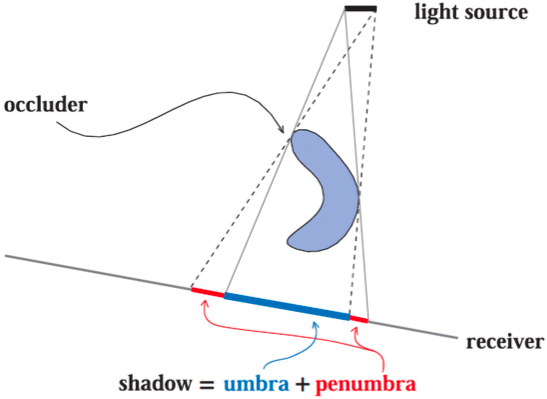
\includegraphics[width=7cm]{shadow.png}
\end{center}
\vspace{.3cm}
Furthermore, shadows convey 3D information of an object, such as:

\begin{itemize}
	\item Relative position
	\item Depth information
	\item Position of the light sources
\end{itemize}
Shadows can be computed by extending the Phong model as follows:

\[ I = I_e + \rho_a \cdot I_a + \sum^n_{j = 1} (\rho_d \cdot \langle n, l_j \rangle + \rho_s \cdot \langle r_j, v \rangle^k) \cdot I_j \cdot \text{attr}(t) \cdot s_j(p) \] \\
Where $s_j(p)$ is either 0 or 1. It is 1 when the secondary ray reaches the light source, 0 if the secondary ray hits another object before reaching the light source.

\subsection{Reflection}
Reflection happens when a ray hits a reflective object. \\

\begin{center}
	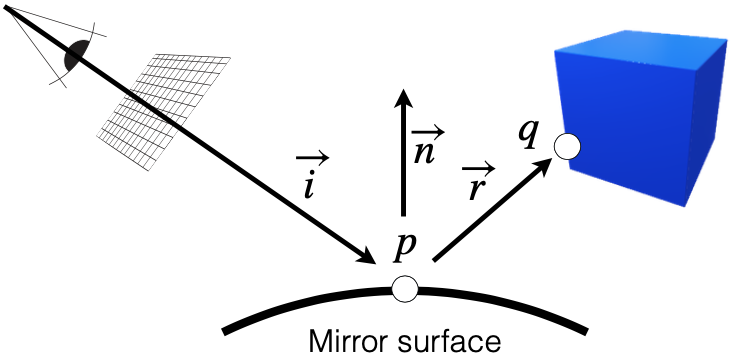
\includegraphics[width=7cm]{reflec.png}
\end{center}
\vspace{.3cm}
In order to compute the reflected vector $r$, we use the following formula:

\[ r = i - 2n \cdot \langle n, i \rangle \] \\
In order to colour the mirror surface, we first need to find the intersection at $q$. The color at point $q$ is then computed and used for $p$ as well. \\ \\
In order to determine how reflective a surface is, we need to use the constant

\[ \alpha_{\text{reflect}} \in [ 0, 1 ] \]

\subsection{Snell's Law}
This law says that the ratio of the sines of the two angles is equal to the ratio of the indices of refraction. This is also equal to the ratio of the velocities in the mediums.

\[ \frac{\sin \Theta_1}{\sin \Theta_2} = \frac{\delta_1}{\delta_2} = \frac{v_1}{v_2} \] \\
We also have that:

\[ \frac{\delta_1}{\delta_2} \cdot \sin \Theta_1 \begin{cases} < 1 & \text{refraction} \\ = 1 & \text{critical angle} \\ > 1 & \text{total internal reflection} \end{cases} \]

\subsection{Refraction}
Refraction happens whenever a ray passes the boundary between two transparent materials. \\

\begin{center}
	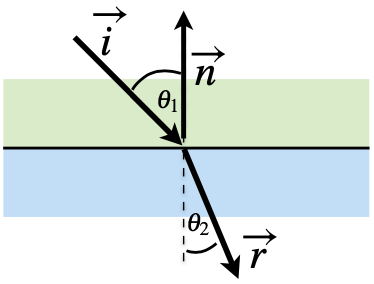
\includegraphics[width=4cm]{refrac.png}
\end{center}
\vspace{.3cm}
The refracted ray $r$ can be found by using the following algorithm:
\begin{align*}
	a &= n \cdot \langle n, i \rangle \\
	b &= i - a \\
	\beta &= \frac{\delta_1}{\delta_2} \\
	\alpha &= \sqrt{1 + ( 1 - \beta^2) \frac{||b||^2}{||a||^2}}
\end{align*}
Where $\delta_1$ and $\delta_2$ are the two indices of refraction of the two materials. And finally

\[ r = \alpha a + \beta b \]

\subsection{Fresnel Effect}
The amount of light that is reflected of refracted on a surface depends on the viewing angle. \\

\begin{center}
	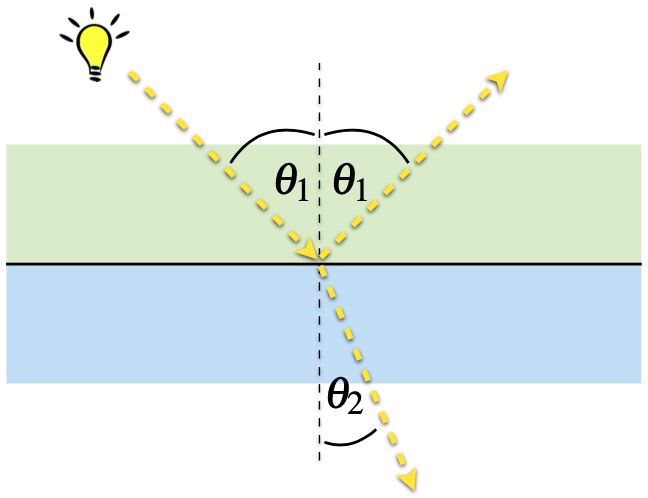
\includegraphics[width=4.5cm]{fresnel.png}
\end{center}
\vspace{.3cm}
The reflected and refracted rays of the Fresnel effect is computed as:

\[ F_{\text{Rl}} = \frac{1}{2} \left( \left( \frac{\delta_2 \cos\Theta_1 - \delta_1 \cos \Theta_2}{\delta_2 \cos\Theta_1 + \delta_1 \cos \Theta_2} \right)^2 + \left( \frac{\delta_1 \cos\Theta_1 - \delta_2 \cos \Theta_2}{\delta_1 \cos\Theta_1 + \delta_2 \cos \Theta_2} \right)^2 \right) \]
\[ F_{\text{Rf}} = 1 - F_{\text{Rl}} \]

\subsection{Space Partitioning}
\textbf{Octrees} are adptive grid subdivisions. They are difficult to traverse. \\ \\
In \textbf{Bounding Volume Hierarchy} (BVM), neighbouring objects are gathered using simple bounding primitives. the gathering difficulty is optimal. When we traverse we start from the biggest primitives. \\ \\
\textbf{Binary Space Partitioning trees} (BSPt) recursively divide the scene with planes. It has a running time of $O(\log n)$, but it is complicated to traverse.

\subsubsection{Kd-Trees}
Here we recursively divide the scene into planes. Differently from BSPt, the planes are axis-aligned. \\ \\
In order to traverse a kd-tree, we use the parametric ray equation

\[ \gamma(t) = o + td \] \\
And we recursively consider the active ray segment

\[ [t_{\min}, t_{\max} ] \] \\
This algorithm runs in $O(\log n)$.

\section{Line Rasterization}
In rasterization, we use the inverse approach of raytracing. The line here is transformed from global coordinates into screen coordinates. The following is the algorithm:

\begin{enumerate}
	\item Consider rays from points $p_1$ and $p_2$ to the origin
	\item Compute the intersections with the image plane at $z = 1$
	\item We now have screen coordinates $(x_1, y_1)$ and $(x_2, y_2)$ for points $p_1$ and $p_2$
	\item Draw the line from $(x_1, y_1)$ to $(x_2, y_2)$
\end{enumerate}
\vspace{.0cm}
\begin{center}
	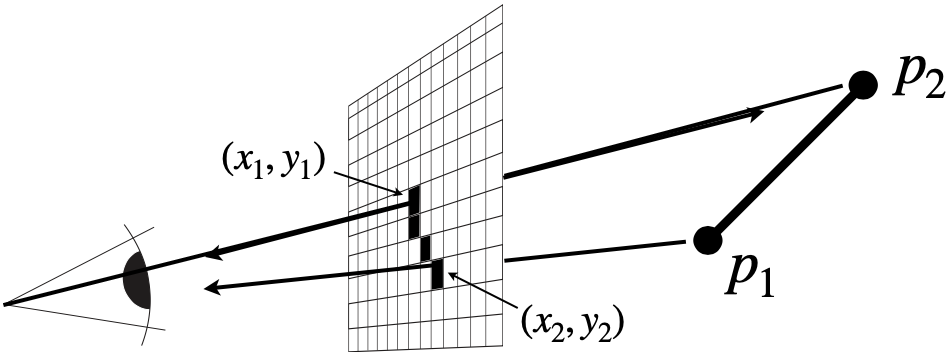
\includegraphics[width=7cm]{rasterization.png}
\end{center}
\vspace{.3cm}
In order to determine which pixels should be coloured in the image, we use the midpoint algorithm.

\subsection{Midpoint Algorithm}
There are two possible options for the selection of the $y$-coordinate at each $x$-step:

\begin{itemize}
	\item Value of $y$ stays the same
	\item Value of $y$ increases by one
\end{itemize}
The following is the decision: \\
\begin{center}
	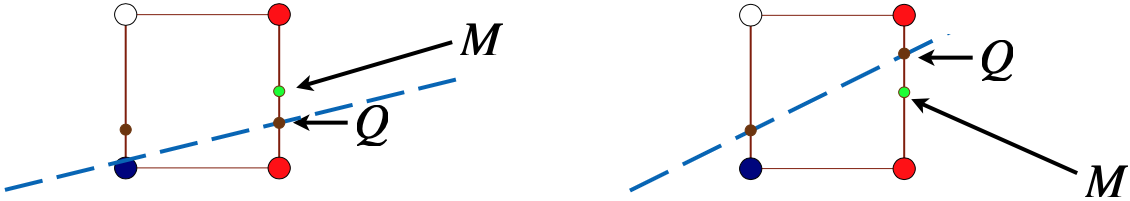
\includegraphics[width=11cm]{midpoint.png}
\end{center}
\vspace{.3cm}
Where $Q$ is the intersection, and $M$ is the midpoint. If $Q$ is higher than $M$, then $y$ will be increased. Otherwise, $y$ stays the same. \\ \\
In order to determine whether a point lies above or below a line, we use the following function:

\[ F(x,y) = ydx - xdy + x_1dy - y_1dy \] \\
Where

\[ dx = x_2 - x_1 \]
\[ dy = y_2 - y_1 \] \\
Now we can check the sign of $F(x,y)$.
\begin{align*}
	F(x, y) \begin{cases} > 0 & \text{above the line} \\ = 0 & \text{on the line} \\ < 0 & \text{below the line} \end{cases}
\end{align*}
From what discussed above, we can have a midpoint decider:

\[ f = F(M) = F(x_i + 1, y_i + 0.5) \] \\
Where, if

\[ f \geq 0 ~~~~~~~~ \text{choose the pixel below} \]
\[ f < 0 ~~~~~~~~ \text{choose the pixel above} \] \\
The initial value for $F(M)$ is:

\[ F(M) = -dy + \left(\frac{dx}{2}\right) \]

\section{Graphics Pipeline}
The steps of the pipeline are:

\begin{enumerate}
	\item \textbf{Application}
	\vspace{.2cm} \\
	It determines the composition of the scene, and is usually computed on the CPU. For example, it sets up the camera, changes geometry, performs animations...
	
	\item \textbf{Geometry Processing}
	\vspace{.2cm} \\
	All of the geometry is put in a common space. the per-vertex shading information is computed. Some of the information is passed to the rasterization stage.
	
	\item \textbf{Rasterization}
	\vspace{.2cm} \\
	Fragments are generated with interpolated per-vertex data.
	
	\item \textbf{Pixel Processing}
	\vspace{.2cm} \\
	Each fragment is coloured. All fragments are merged into an image.
\end{enumerate}
\subsection{Detailed Pipeline}
There are more detailed steps in the rendering pipeline:

\begin{enumerate}
	\item \textbf{Vertex Specification}
	\vspace{.2cm} \\
	Setting up the geometry. It is a \textbf{fixed stage}.
	
	\item \textbf{Vertex Shader}
	\vspace{.2cm} \\
	Computes the transformation and shading info. It is a \textbf{programmable stage}.
	
	\item \textbf{Tesselation}
	\vspace{.2cm} \\
	Subdivides geometry. It is a \textbf{programmable stage}.
	
	\item \textbf{Geometry Shader}
	\vspace{.2cm} \\
	Generates the new geometry. It is a \textbf{programmable stage}
	
	\item \textbf{Vertex Post-Processing}
	\vspace{.2cm} \\
	Performs clipping and outputs the geometry. It is a \textbf{fixed stage}.
	
	\item \textbf{Primitive Assembly}
	\vspace{.2cm} \\
	Creates a geometry from vertices, and performs face culling. It is a \textbf{fixed stage}.
	
	\item \textbf{Rasterization}
	\vspace{.2cm} \\
	Creates the fragments, and performs data interpolation. It is a \textbf{fixed stage}.
	
	\item \textbf{Fragment Shader}
	\vspace{.2cm} \\
	Performs shading. It is a \textbf{programmable stage}.
	
	\item \textbf{Pre-Sample Operations}
	\vspace{.2cm} \\
	Perform depth testing. It is a \textbf{fixed stage}.
\end{enumerate}

\subsection{Data Flow}
\textbf{Uniforms} are input data common across all shader executions. They can be numbers, vectors, textures... \\ \\
\textbf{Attributes} are per-vertex input information, such as color, position... These values are interpolated and stored inside of buffers. \\ \\
\textbf{Fragment values} are optional, and usually represent color information. \\

\begin{center}
	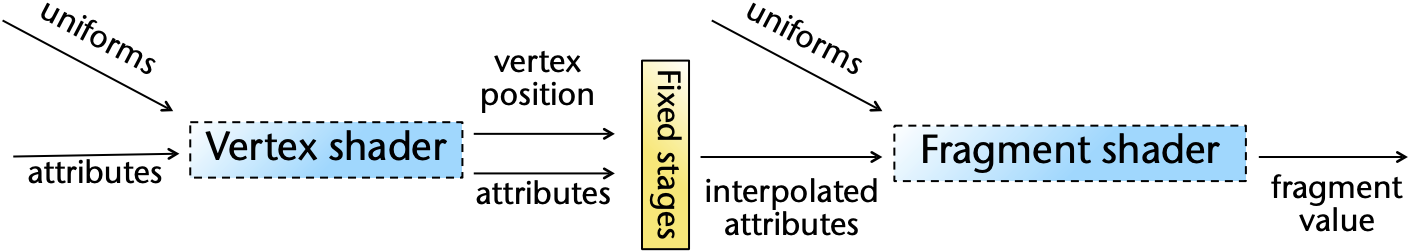
\includegraphics[width=11cm]{data_flow.png}
\end{center}

\subsection{Supplying Vertex Attributes}
Geometric objects are stored as vertices. A \textbf{vertex} is a simple collection of attributes in space. These attributes are:

\begin{itemize}
	\item Position
	\item Colour
	\item Normal vector
\end{itemize}
This vertex data is stored into buffers called \textbf{vertex buffer objects} (VBOs). VBOs are concatenated elements of each vertex. \\ \\
On the other hand, \textbf{Vertex Array Objects} (VAOs) describe the state of the attributes, which VBO to use, and how to pull the data from it.

\subsection{Depth Test and Face Culling}
The \textbf{depth test} is necessary in order to find which object occludes which other object. \\ \\
\textbf{Face culling} allows to prevent the rendering of the faces that are not visible to the viewer.

\section{Transformation Pipeline}
\subsection{Model Transformation}
It transforms model coordinates into world coordinates. It is defined by a \textbf{model matrix} representing affine transformations.

\subsection{Viewing Transformation}
It transforms world coordinates into viewing coordinates. It is computed as:
\begin{align*}
	eye &= VP \\
	z' &= \frac{VPN}{||VPN||} \\
	x' &= \frac{VUP \times z'}{||VUP|| \times z'||} \\
	y' &= z' \times x'
\end{align*}
Where $VP$ is the camera position, $VPN$ is the view plane normal, and $VUP$ is the view up vector. Then:

\[ T(-eye) = \begin{bmatrix} 1 & 0 & 0 & -eye_x \\ 0 & 1 & 0 & -eye_y \\ 0 & 0 & 1 & -eye_z \\ 0 & 0 & 0 & 1 \end{bmatrix} \]
\[ p = p'_xx' + p'_yy' + p'_zz' = Rp' \]
\[ R = \begin{bmatrix} \vline & \vline & \vline & 0 \\ x' & y' & z' & 0 \\ \vline & \vline & \vline & 0 \\ 0 & 0 & 0 & 1 \end{bmatrix} \]
\[ p' = R^{-1}p = R^Tp \] \\
Finally, the \textbf{view matrix} will be:

\[ R^TT(-eye) = \begin{bmatrix} - & x^T & - & -x'^T \cdot eye \\ - & y^T & - & -y'^T \cdot eye \\ - & z^T & - & -z'^T \cdot eye \\ 0 & 0 & 0 & 1 \end{bmatrix} \]

\subsection{Projection Transformation}
It transforms viewing coordinates to normalized coordinates. In order to do so, we need to use an orthographic projection. \\ \\
In order to perform an orthographic projection, we need to transform a map cuboid into a unit cube. This is done with the \textbf{projection matrix}.

\[ P_{ortho} = \begin{bmatrix} \frac{1}{r} & 0 & 0 & 0 \\ 0 & \frac{1}{t} & 0 & 0 \\ 0 & 0 & \frac{-2}{f-n} & -\frac{f+n}{f-n} \\ 0 & 0 & 0 & 1 \end{bmatrix} \]

\subsection{Transformations for Rasterization}
The final formula for the transformations of vertices is:

\[ out = PM \cdot VM \cdot MM \cdot in \] \\
Where $PM$ is the projection matrix, $VM$ is the view matrix, $MM$ is the model matrix, and $in$ is the input vertex.

\section{Light Computation}
The Phong reflectance model can be used in rasterization by the following formula:

\[ I = k_ai_a + k_d (L \cdot N) i_d + k_s (R \cdot V)^s i_s \] \\
Where $k_a$ is the ambient coefficient, $i_a$ is the ambient intensity, $k_d$ is the diffuse coefficient, $L$ is the vector pointing to the light source, $N$ is the normal vector of the intersection point, $i_d$ is the diffuse intensity, $k_s$ is the spectral coefficient, $R$ is the reflected vector, $V$ is the vector pointing to the viewer, $s$ is the shininess of the object, and $i_s$ is the spectral intensity.

\subsection{Shading}
There are two main techniques in order to compute the color of a point:

\begin{itemize}
	\item \textbf{Gouraud Shading}
	\vspace{.2cm} \\
	The color is computed per-vertex and is then interpolated. The Phong model computation is done in the vertex shader.
	
	\item \textbf{Phong Shading}
	\vspace{.2cm} \\
	All the information for light computation is first interpolated. It is computed in the fragment shader.
\end{itemize}
Each fragment is shaded separately in a fragment shader. All vectors should be available there. \\ \\
The available vectors are:

\begin{itemize}
	\item \textbf{Normal vector - $N$}
	\vspace{.2cm} \\
	It contains geometry information and is transformed using model and view matrices.
	
	\item \textbf{Light vector - $L$}
	\vspace{.2cm} \\
	This vector can be either passed to the vertex shader and transformed with a view matrix, or it can be transformed with a view matrix in the application stage.
	
	\item \textbf{View direction - $V$}
	\vspace{.2cm} \\
	It is easy to compute, since the camera is located in $(0, 0, 0)$. It can be computed in the vertex shader from the vertex position transformed by both the model and the view matrices.
	
	\item \textbf{Reflection direction - $R$}
	\vspace{.2cm} \\
	It can be computed in the fragment shader from vectors $L$ and $N$.
\end{itemize}

\section{Textures}
\subsection{Texture Mapping}
A 3D texture is composed by the following layers:

\begin{itemize}
	\item Diffuse colour
	\item Normal
	\item Roughness
	\item Displacement
	\item Ambient occlusion
\end{itemize}
Non-parametric surfaces can be textured with different techniques, such as:

\begin{itemize}
	\item Box mapping
	\item Cylindrical mapping
	\item Planar mapping
\end{itemize}

\subsection{UV Unwrapping}
Some surfaces, which are called deployable surfaces, can be flattened. Some problems can arise from UV unwrapping, such as:

\begin{itemize}
	\item \textbf{Area Distortion}
	\vspace{.2cm} \\
	The same texture size can be applied to different sizes in 3D, or the opposite.
	
	\item \textbf{Angle Distortion}
	\vspace{.2cm} \\
	The same texture shape can be used for different shapes in 3D.
\end{itemize}
The seams generated by UV unwrapping can be hidden in sharp edges or non-visible areas.

\subsection{Texturing in the Graphic Pipeline}
First, we need to interpolate (u,v) from UVs of the vertices. The corresponding value is fetched from the texture. UVs are new attributes in the vertex shader. \\ \\
The interpolation of these points is done in the GPU.

\subsection{Mip-Mapping}
Here we have a texture hierarchy with textures at smaller sizes too. This means that one third more texture space is required.

\subsection{Normal Mapping}
Normal mapping is done in order to reflect light off of a coarse geometry.

\[ \overrightarrow{N}_{new} = \begin{bmatrix} n_x \\ n_y \\ n_z \end{bmatrix} = 2 \begin{bmatrix} R \\ G \\ B \end{bmatrix} - \begin{bmatrix} 1 \\ 1 \\ 1 \end{bmatrix} \] \\
In order to handle arbitrary geometry, the normal has to be defined in the local coordinate system.

\subsection{Tangent Space}
We need a normal, tangent and bitangent in order to transform normals from the texture coordinate system to a different coordinate system.

\[ P_i - P_j = \langle (U_i - U_j), T \rangle + \langle (V_i - V_j), B \rangle \] \\
Where $T$ is the tangent and $B$ is the bitangent.

\[ T = T - \langle N, T \rangle \cdot N \]
\[ B = N \times T \] \\
Where $\times$ is the cross product operator and $\langle ~ \rangle$ is the dot product operator. Make also sure that:

\[ \langle B, N \times T \rangle > 0 \] \\
The computed normal needs to be substituted to the previous geometry normal.

\subsection{Skybox}
This is a cube centred around the origin $(0,0,0)$ and surrounds the scene. \\ \\
In order to find the environment colour, we need to perform \textbf{environment mapping}.

\begin{center}
	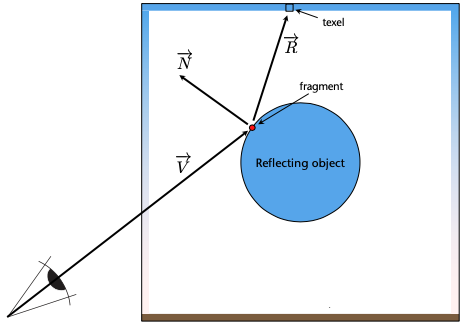
\includegraphics[width=7cm]{skybox.png}
\end{center}
\vspace{.3cm}
First of all we compute the view direction. then we reflect according to the normal. We now fetch the value of the cube map using the reflected direction.

\section{Shadows in Rasterization}
The problem for shadows in rasterization, is that their computation is a global type of problem. Any two objects in the scene could potentially shadow each other. \\ \\
In order to solve the above problem, we can use some sort of pre-processing strategy, as well as looking the scene from the point of view of the light source.

\subsection{Shadow Maps}
A point is in shadow of some object if some other object point is closer to the light source. \\

\begin{center}
	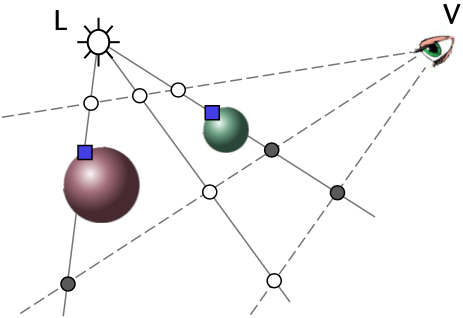
\includegraphics[width=7cm]{shadow_map.png}
\end{center}
\vspace{.3cm}
Where the \textit{blue squares} are the intersections of the light rays with the objects, the \textit{white circles} are the points in which there is no shadow, and the \textit{gray circles} are the points in which there is shadow. \\ \\
In the pre-processing phase, all object points that are closest to the light source $L$ are computed. Afterwards, during rendering, we test the current distance to $L$ with the stored smallest distance.

\subsubsection{Pre-Processing}
Scenes are rendered as seen from the light source $L$. The resulting $z$-buffers will contain the smallest distance $z_{min}$ of the object point to $L$. \\ \\
The $z$-buffers are used as \textbf{shadow maps}. \\ \\
The fragments' 3D coordinates are transformed into the local coordinate system of the light source. A fragment is said to be in shadow, iff:

\[ z > z_{min} \]

\subsubsection{Rendering}
First we render the scene as seen from the light source. One shadow map is created for each light source. \\ \\
Then we render the scene from the viewing point $V$. Here a per-fragment computation is carried out:

\begin{itemize}
	\item If $z < z_{min}$, then we use only the ambient term in order to compute the color of the point
	\item Otherwise, we have normal full lighting
\end{itemize}

\subsection{Off-Screen Rendering}
In order to carry out render-to-texture, we need to create a \textbf{Frame Buffer Object} (FBO). In this FBO we put the shadow texture, and then bind it. After doing so, we unbind the FBO and use its textures as regular textures.

\subsection{Shadow Map Artefacts}
\subsubsection{Shadow Acne}
When comparing the shadow map values with vertex depth, we could run into precision issues. \\ \\
In order to fix this, we add a tiny bias ($\sim 0.001$).\\

\begin{center}
	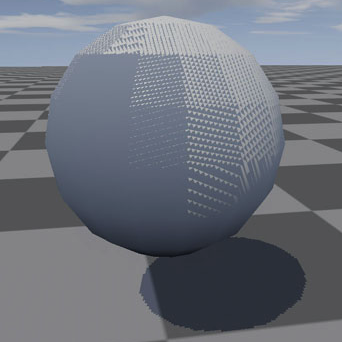
\includegraphics[width=4cm]{shadow_acne.png}
\end{center}

\subsubsection{Undersampling}
Perform comparisons with the shadow map in multiple small neighbourhoods. Set the shadowing to the percentage of neighbours that are in shadow.

\end{document}